\section{Stochastic Routing Methodology}

The principle of stochastic optimization is to find the set of controls which returns the best expected outcome for an uncertain situation modeled as a set of discrete situations of known likelihood. The goal of stochastic optimization is

\begin{equation}
	\min_{\overline{U}}\quad J(U)=\sum_{S\in\overline{S}} P(S)F(U,S)\label{eq:stochastic_optimization}
\end{equation}

where $\overline{S}$ is the set of possible scenarios, $P(S)$ is the probability of $S$, $F(U,S)$ is the cost of control vector $U$ for scenario $S$, and $\overline{U}$ is the set of possible controls. A control vector $U=\{U_g,U_p\}$ contains general and specific controls (sometimes called first and second stage controls). General controls are shared among all scenarios and specific controls apply only ot one scenario. An example of stochastic optimization is provided in the Appendix.

For a \gls{bev} driving between an origin and a destination the controls relate to where to charge. If there is less than 100\% certainty of a charger being usable (functional, accessible, and available) at the time of arrival to the charger, the optimization becomes stochastic. The technical non-functionality of a given charger may be known to the driver before the trip but accessibility and availability are not likely to be known prior to arrival. When a driver arrives at a charger and becomes aware that the charger is not usable the driver has the following options: (1) Wait at the charger until it becomes available, (2) re-route from current location to destination. If the charger is found to be non-functional or inaccessible then only option (2) is possible. Less than perfect reliability may result in an optimal route which is, otherwise, higher cost than that for perfect reliability. Less than perfect certainty may result in a route which is, otherwise, higher cost than that produced with perfect information. Sufficiently poor reliability/certainty may render a trip infeasible from the start or after several failed charge events.

\subsection{Algorithms}

Where deterministic routing occurs on a graph $G$, stochastic routing occurs on the spanning set of possible graphs $\overline{G}$ which has infinite cardinality in which all graph are isomorphic to all others ($G_i \cong G_j \ \forall \ i,j \in\hat{G}$). A corollary is that producing a route for $\overline{G}$ requires that there is some flat bijection $f:V_G\rightarrow V_H$ such that $(u,v)\in E_G \iff (f(u),f(v))\in E_H\ \forall u, v \in V_G$ common to all graphs in $\overline{G}$ which contains the primary structure of the graph (which nodes and links are present). The flat isomorphic graph is $G' = \{V', E'\}$. Variability in route cost is caused by the differences in non-primary node and edge properties between graphs. An example would be a road network where the streets are always present but have variable speeds, some of which may be zero, at a given time.

In reality, optimization must occur over a finite set. Thus stochastic optimization occurs on $\hat{G}\subset\overline{G}$ of cardinality $N$. Higher values of $N$ better approximate $\overline{G}$ at the cost of increased computational load. Dijkstra's method for stochastic routing results in a single general optimal route $R^*$. $R^*$ is found using a Monte-Carlo style solution wherein $N$ integrations are simultaneously computed along the same paths experiencing different parameters along the way. The goal of the optimization is to produce the route with the lowest expected cost $\mathbb{J}^* = F(R^*,\hat{G})$ where $R^*$ is the expected optimal route.

$R^*$ is subject to charger usability for O/D pairs of a greater distance than the vehicle's remaining range. The net result of charging (or fueling etc.) is that the vehicle's range is reset, time is added to the route, and money is added to the route price. Time additions are due to charge time and a possible delay due to queuing. Price additions are due to charge pricing. As such, the chargers in $\hat{G}$ (present at a subset of nodes $V'_C$) are defined by function $\Theta$ whose parameters are $\hat{\Psi} = \{\Psi_G,\quad \forall G\in \hat{G}\}$ where $\Psi_G = \{\psi_v^r,\psi_v^p,\psi_v^d,\psi_v^c\ \ \forall v\in V'_C\}$. The parameters of $\Theta$ are the range completion of the charge event (the reset range), the charge power, the wait time before charging, and the charging cost respectively. If the vehicle's remaining range is greater than $\psi_v^r$ no charge event will occur. For stochastic optimization, all parameters are sampled from defined distributions each time the charger is visited.

Depending on the configuration of $G$, certain routes may be feasible or infeasible (because they cause the vehicle range to go below a minimum value) potentially creating a discontinuous cost space where the costs of the feasible routes must be considered alongside those of infeasible routes. A probabilistic risk measure, the superquantile provides an elegant solution. The superquantile function for a given distribution is

\begin{equation}
	S_p(D) = \frac{1}{1-p}\int_{p}^{1}Q_\alpha(D)d\alpha
\end{equation}

where $D$ is a given \gls{pdf}, $p\in[0, 1]$ is a probability threshold, and $Q_\alpha$ is the quantile function of a given \gls{pdf} for probability $\alpha$. In effect, the superquantile is the mean of the \gls{pdf} after $p$. For route $R$ on graphs $\hat{G}$ of cardinality $N$, there will be a revealed distribution $D_r$ of remaining range at all points. The remaining range constraint can thus be written as

\begin{equation}
	S_p(-D_r)\geq -r^{min} \label{eq:remaining_range_constraint}
\end{equation}

where $r^{min}$ is the lowest allowable remaining range and $p$ is set by the user. In effect, \eqref{eq:remaining_range_constraint} guarantees that the expected value of the worst $1-p$ portion of outcomes is within the feasible range. General values of other route costs are computed similarly. The routing framework described above will be referred to as \gls{scram}.

\subsubsection{\gls{scramd}}

The \gls{scramd} algorithm is outlined below.

\begin{algorithm}[H]
	\caption{\gls{scramd} Routing Algorithm}
	\begin{algorithmic}
		\State $G' = f(G \in \hat{G}) = \{V', E'\}$ \Comment{Flat isomorph common to all graphs in $\hat{G}$}
		\State $\hat{C} = \{\hat{C_V}, \hat{C_E}\}$ \Comment{Costs for graph elements for each graph in $\hat{G}$}
		\State $\hat{\Psi} = \{\Psi_v,\quad \forall v\in V'_C\subset V'\}$ \Comment{Charger parameters for the subset of nodes with chargers in $G'$}
		\State $O\in V'$ \Comment{Single origin node}
		\State $D\in V'$ \Comment{Set of destination nodes}
		\State
		\State $S = \{\}$ \Comment{Set of visited nodes}
		\State $W = \{\{\infty\}_{G \in \hat{G}}\}_{v \in V'}$ \Comment{All node weights initialized to infinity for all graphs}
		\State $R = \{\{\}\}_{d \in D}$ \Comment{Initializing empty path for each destination}
		\State $F = \{(w_{o_0}, o_0)\}$
		\State \Comment{Heap queue containing nodes to be visited. Elements are tuples (weight, node) and the heap is ordered by weight. The heap is initialized with the origin node.}
		\State
		\While {$F\neq \emptyset$} \Comment{Iterate while there are reachable nodes which have not been visited}
		\State $w_v, v = f_0$
		\State $F = F \not\cup f_0$ \Comment{Remove current node from heap queue}
		\If{$v \in V'_C$} \Comment{If current node is a charger ...}
		\State $l_G, w_{v,G} = \theta_G(l_G,w_{v,G},\psi_G)$ \Comment{Update remaining range and cost after charging}
		\EndIf
		\State $E'_v = \{(v_s, v_t)\in E'| v_s = v\}$
		\ForAll{$(v, v_t) \in E'_v$} \Comment{Iterate through links of $v$}
		\State $\mathbb{E}[w_{v_t}] = \mathbb{E}[\{w_v + c_{v,(v, v_t)} + c_{v_t}\}_{G \in \hat{G}}]$ \Comment{Compute an expectation for cost of current path}
		\If{$\mathbb{E}[w_{v_t}] < w_{v_t}$} \Comment{If current path represents savings ...}
		\State $r_{v_t} = r_{v}\cup \{v_t\}$ \Comment{Update path to $v_t$}
		\State $w_{v_t} = \mathbb{E}[w_{v_t}]$ \Comment{Update cost at $v_t$}
		\If{$v_t \not\in S$} 
		\State $F = F \cup \{(w_t, v_t)\}$ \Comment{If $v_t$ has not been visited add to heap queue}
		\EndIf
		\EndIf
		\EndFor
		\State $S = S\cup\{v\}$ \Comment{Add current node to set of visited nodes}
		\EndWhile
	\end{algorithmic}
\end{algorithm}

\subsection{Routing-Based Metrology}

\gls{scram} is valid for any $N$. The added value of \gls{scram} is that is that it allows for risk-tolerance-sensitive routing. This is of particular value for \glspl{pev} because charger usability is not guaranteed. When a \gls{pev} driver arrives at a charger it may be non-functional or inaccessible in which case it cannot be used or unavailable in which case the driver must wait to use it. Non-functionality and inaccessibility are complete failures where unavailability is a partial failure. Complete failures are modeled using $\psi_v^r$. If the vehicle's remaining range is greater than $\psi_v^r$ then the vehicle does not charge, if $\psi_v^r = 0$ then no vehicle can charge which is equivalent to a complete failure. Thus $\psi_v^r$ can be sampled from $\{0, r\}$ with defined probabilities for each. Partial failures are modeled with the $\psi_v^d$ term which is sampled from $[0, \infty)$ and added to the time required for route $R$ which includes $v$. Risk tolerance is modeled using the superquantile function parameter $p \in [0, 1]$ where higher values indicate a tighter focus on worse outcomes. \textbf{Thus $R^*$ is a function of both graph parameter distributions and driver risk tolerance}.

Consider a randomly generated graph of 100 nodes on a 1,000 by 1,000 km grid where chargers are located at 15 nodes. Link probabilities are proportional to distance by the formula $P((v, u)) = \exp(\frac{-\rVert(v, u)\rVert}{s})$ where the characteristic distance $s$ is 200 km. A driver is currently at a single origin node and wants to find $R^*$ for every other node. The driver's car has a range of 400 km. The driver has risk tolerance $p$. Charger parameters are randomly sample as above where the probability of charger complete failure is $\eta$. Risk tolerance applies both the the probability of route completion and the metric of optimization which is travel time in this case. A factorial of cases for $p \in \{.5, .9\}$ and $\eta \in \{.1, .5\}$ are shown in Figure \ref{fig:parameter_factorial}.

\begin{figure}[H]
	\centering
	\begin{subfigure}{.5\linewidth}
		\centering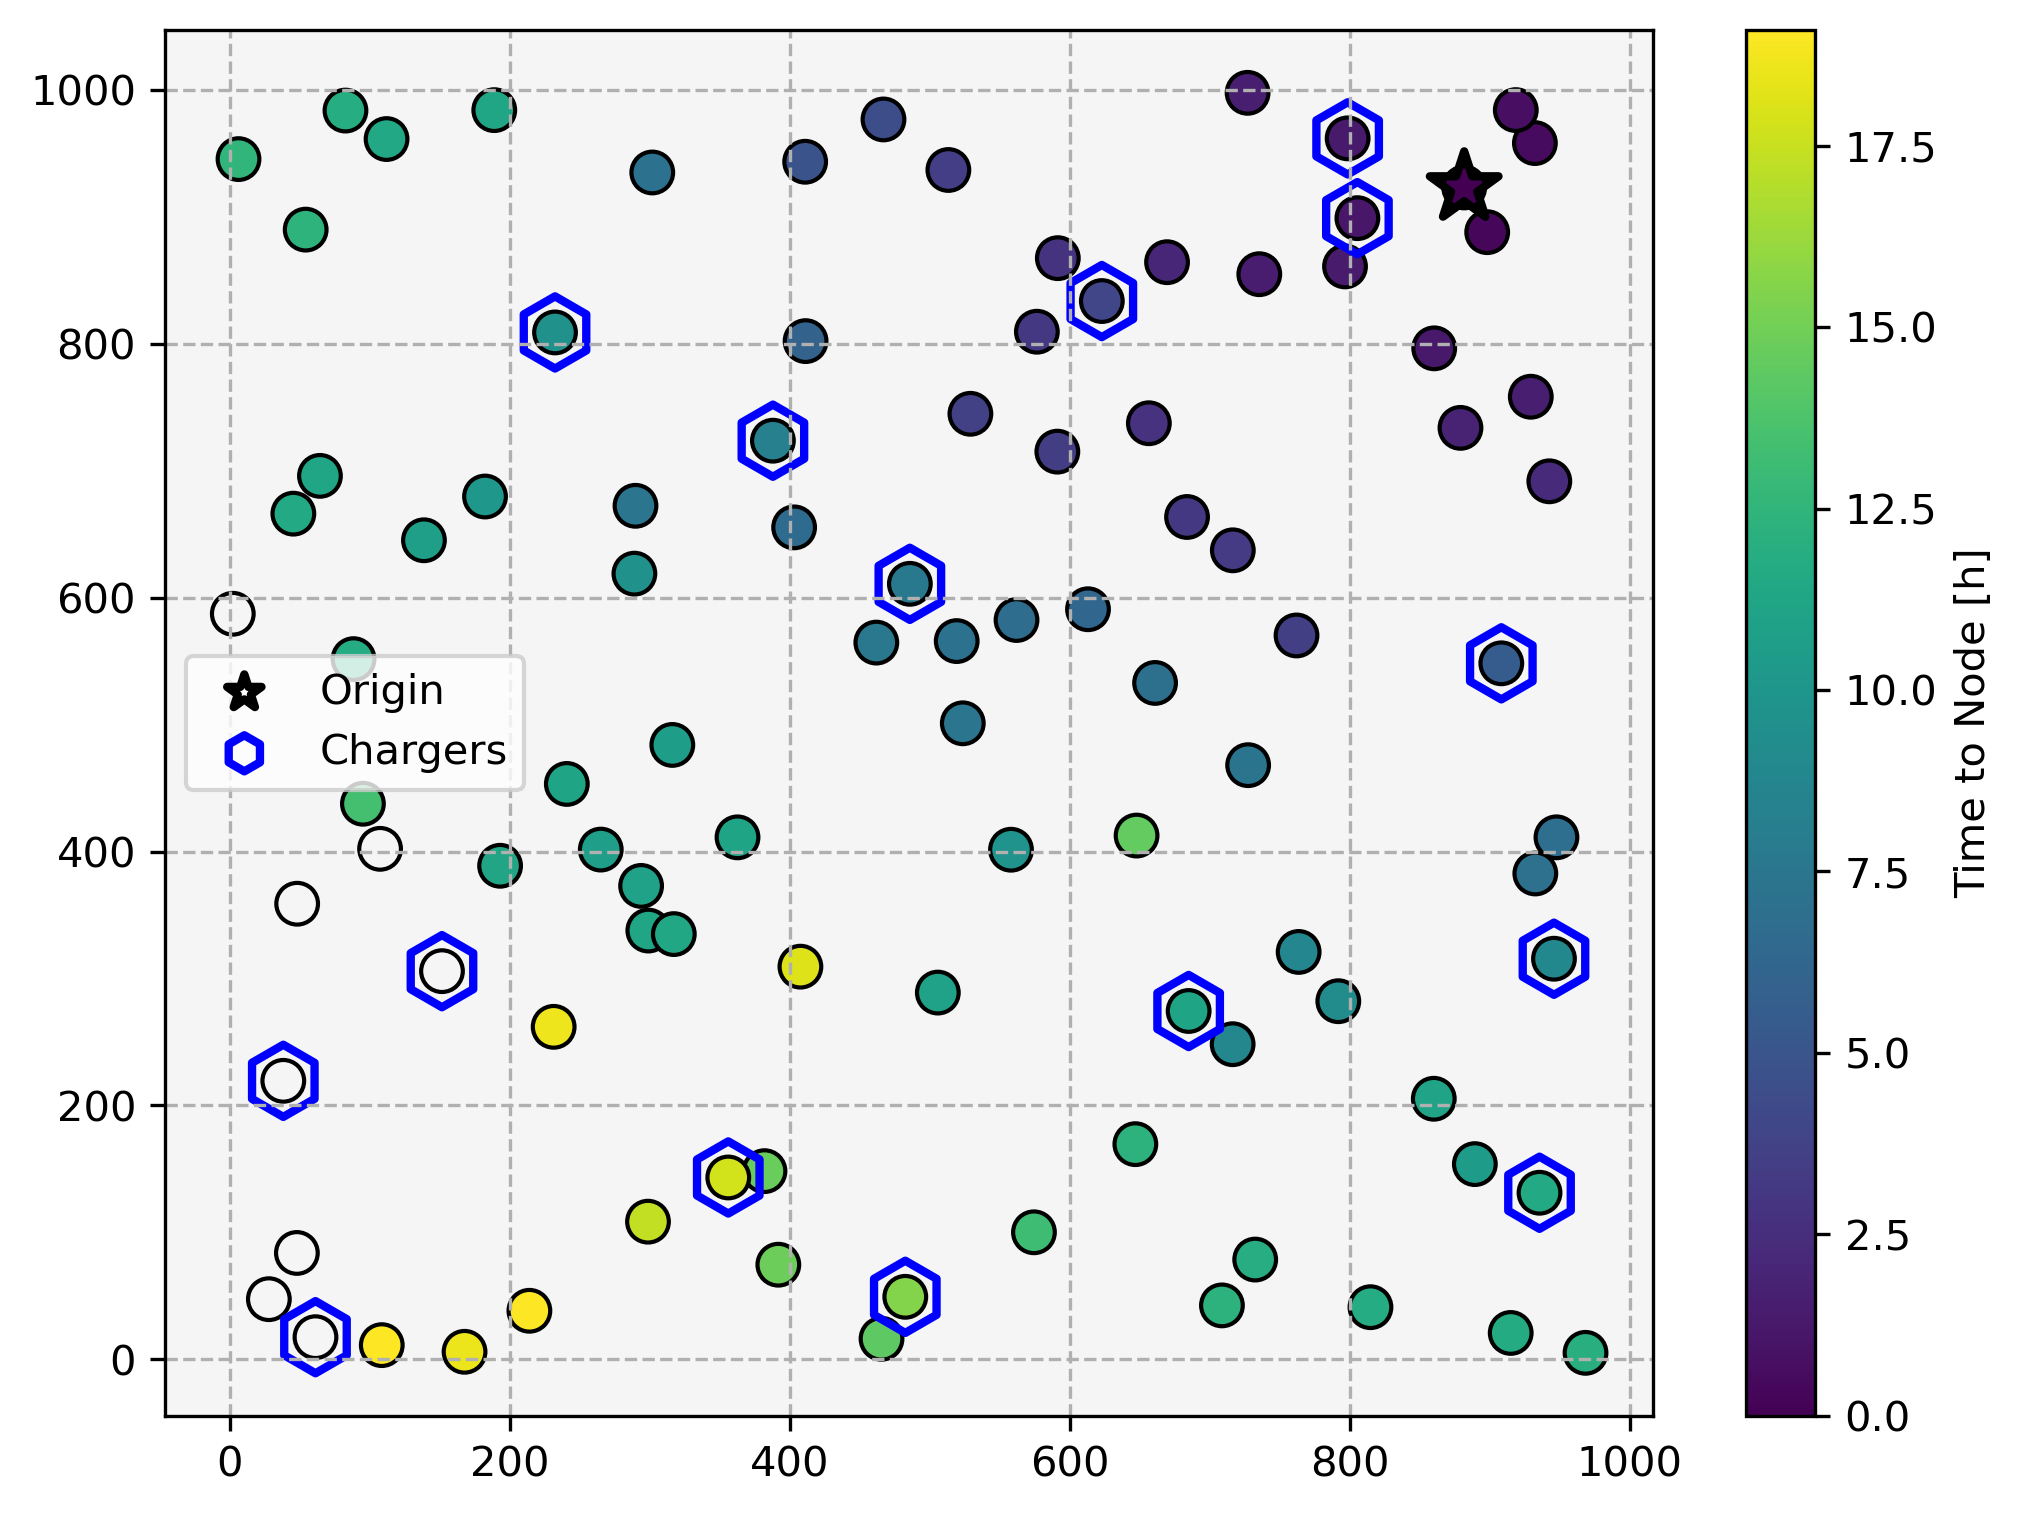
\includegraphics[width = \linewidth]{figs/parameter_factorial_00.png}
		\captionsetup{width=.8\linewidth}
		\caption{High risk tolerance and high charger reliability ($p = .5,\ \eta = .1)$}
	\end{subfigure}%
	\begin{subfigure}{.5\linewidth}
		\centering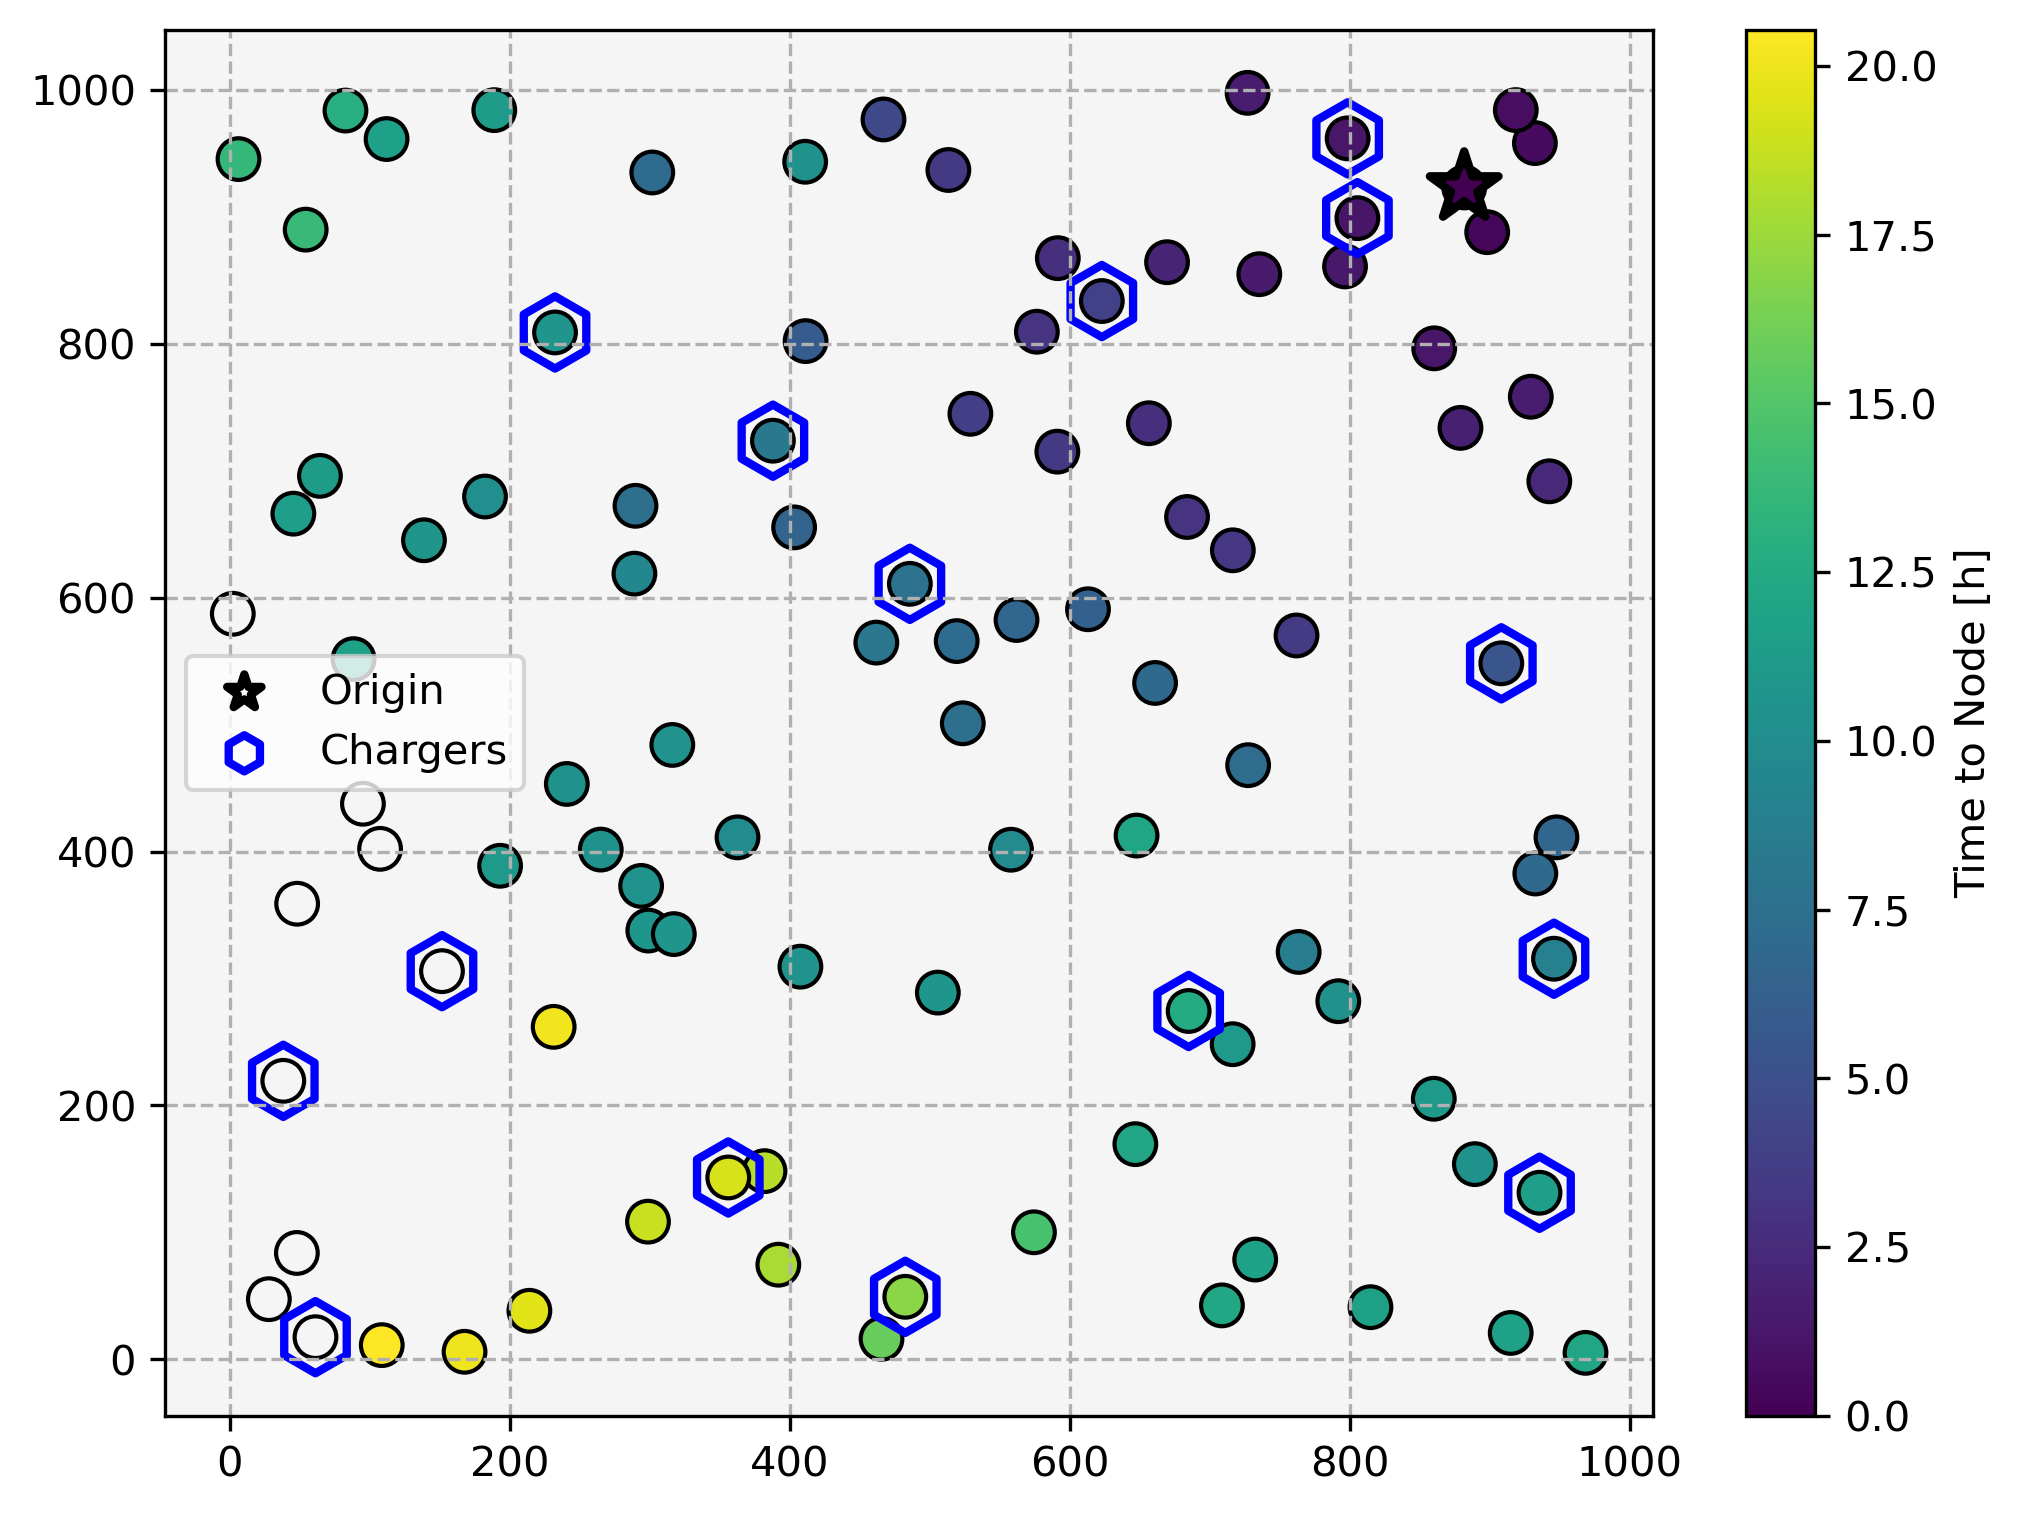
\includegraphics[width = \linewidth]{figs/parameter_factorial_01.png}
		\captionsetup{width=.8\linewidth}
		\caption{High risk tolerance and low charger reliability ($p = .5,\ \eta = .5)$}
	\end{subfigure}
	\begin{subfigure}{.5\linewidth}
		\centering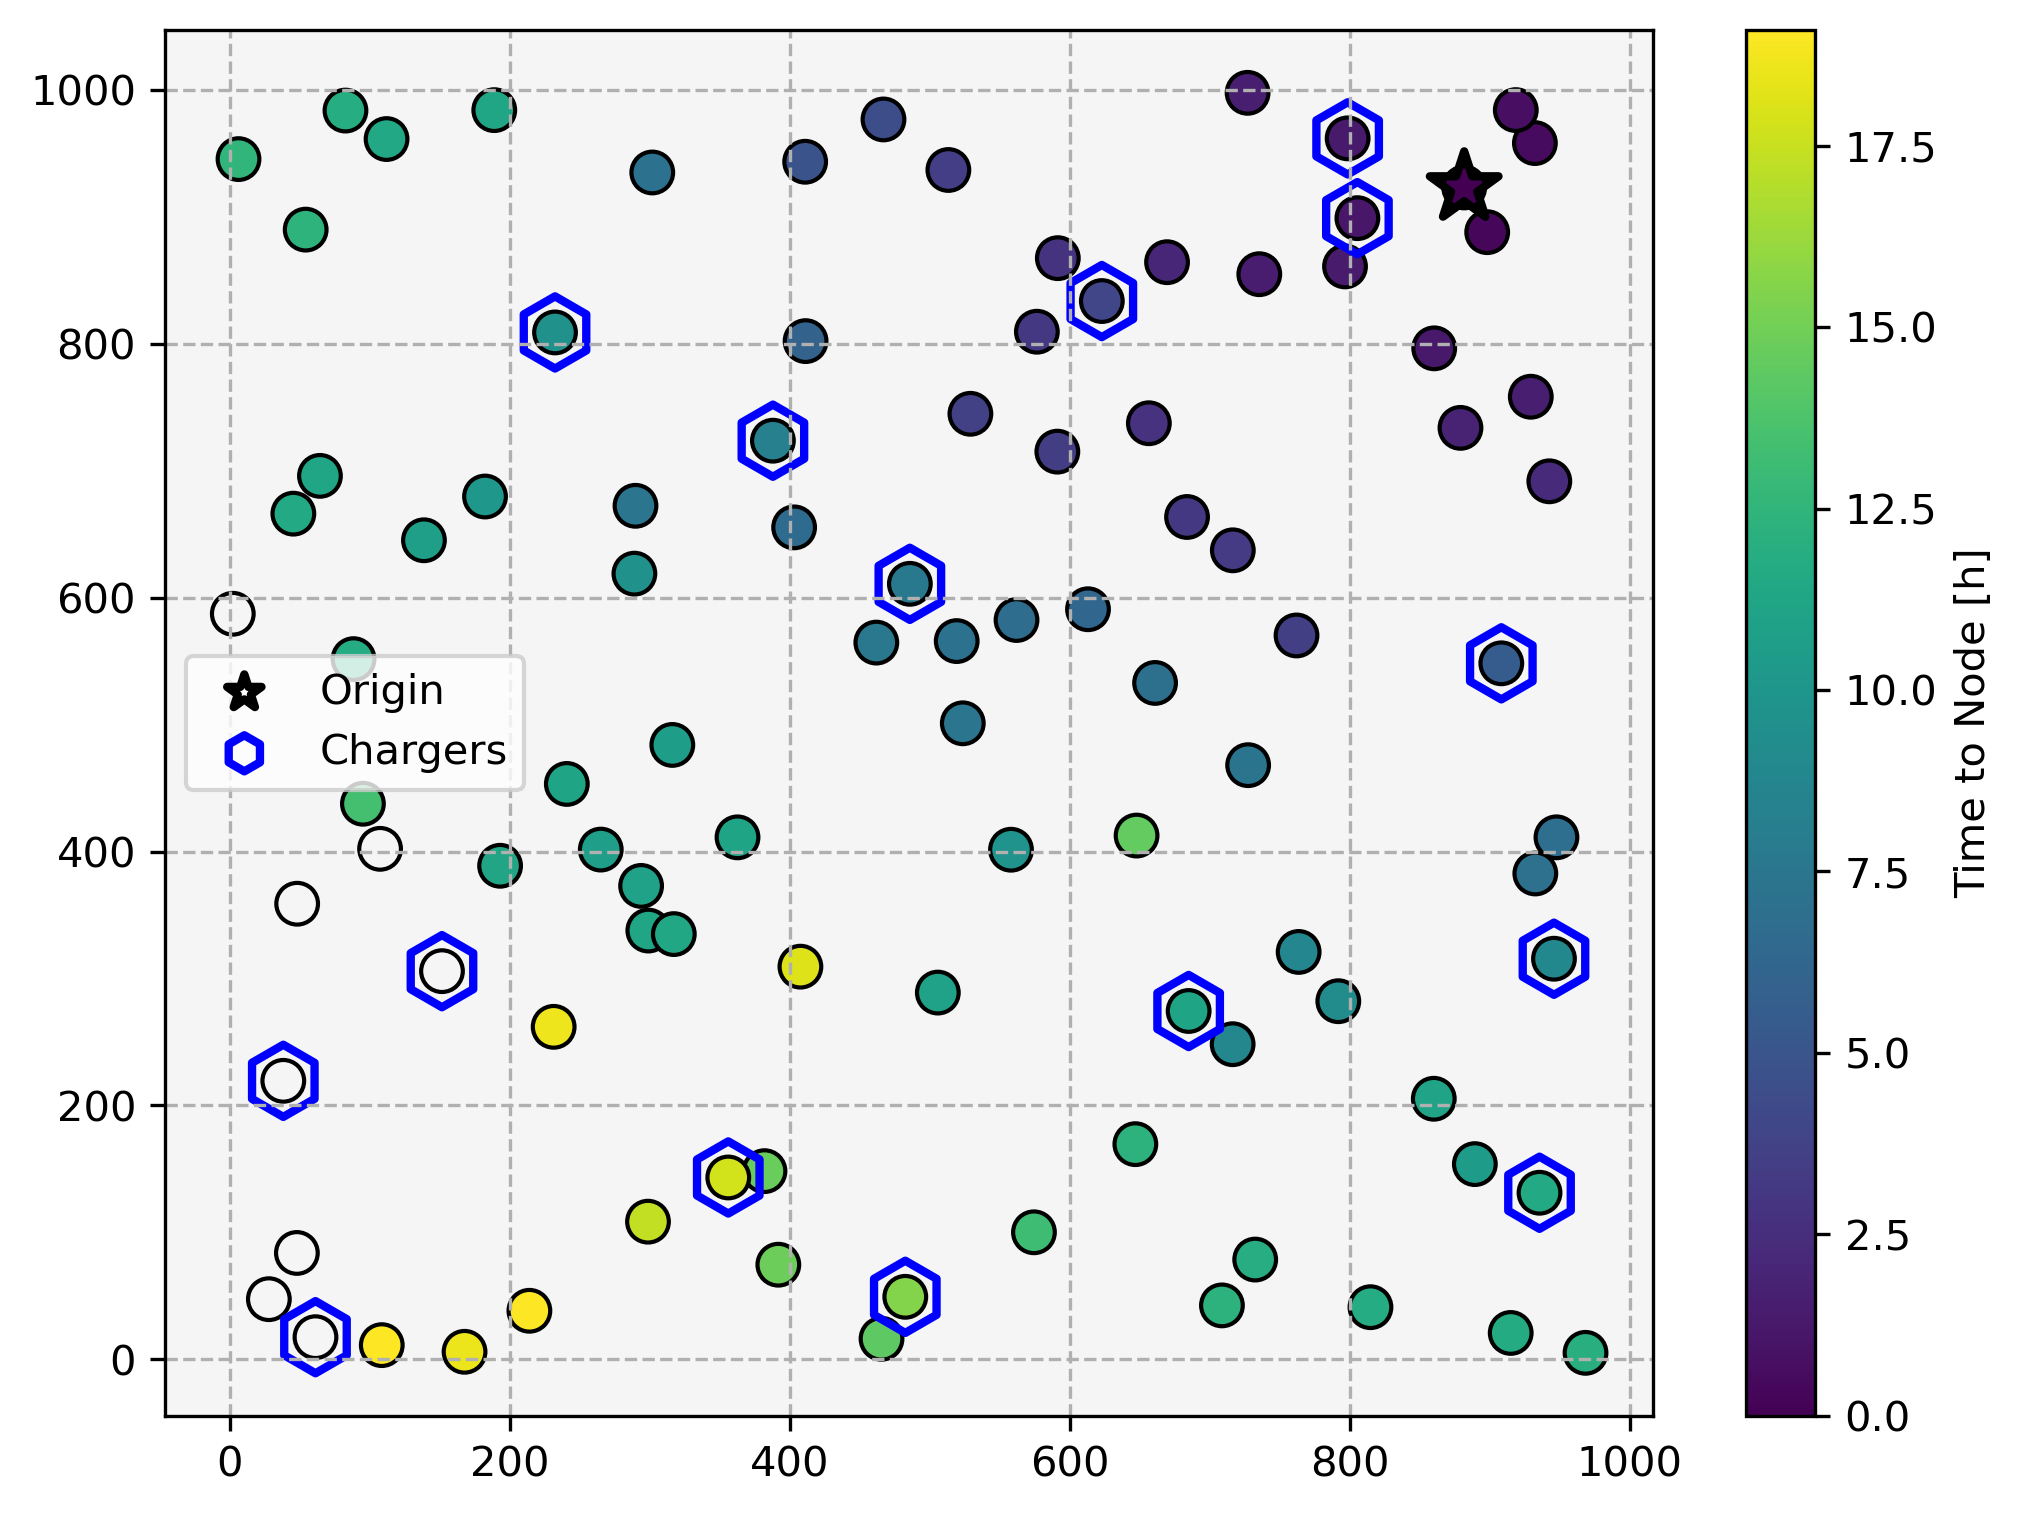
\includegraphics[width = \linewidth]{figs/parameter_factorial_10.png}
		\captionsetup{width=.8\linewidth}
		\caption{Low risk tolerance and high charger reliability ($p = .9,\ \eta = .1)$}
	\end{subfigure}%
	\begin{subfigure}{.5\linewidth}
		\centering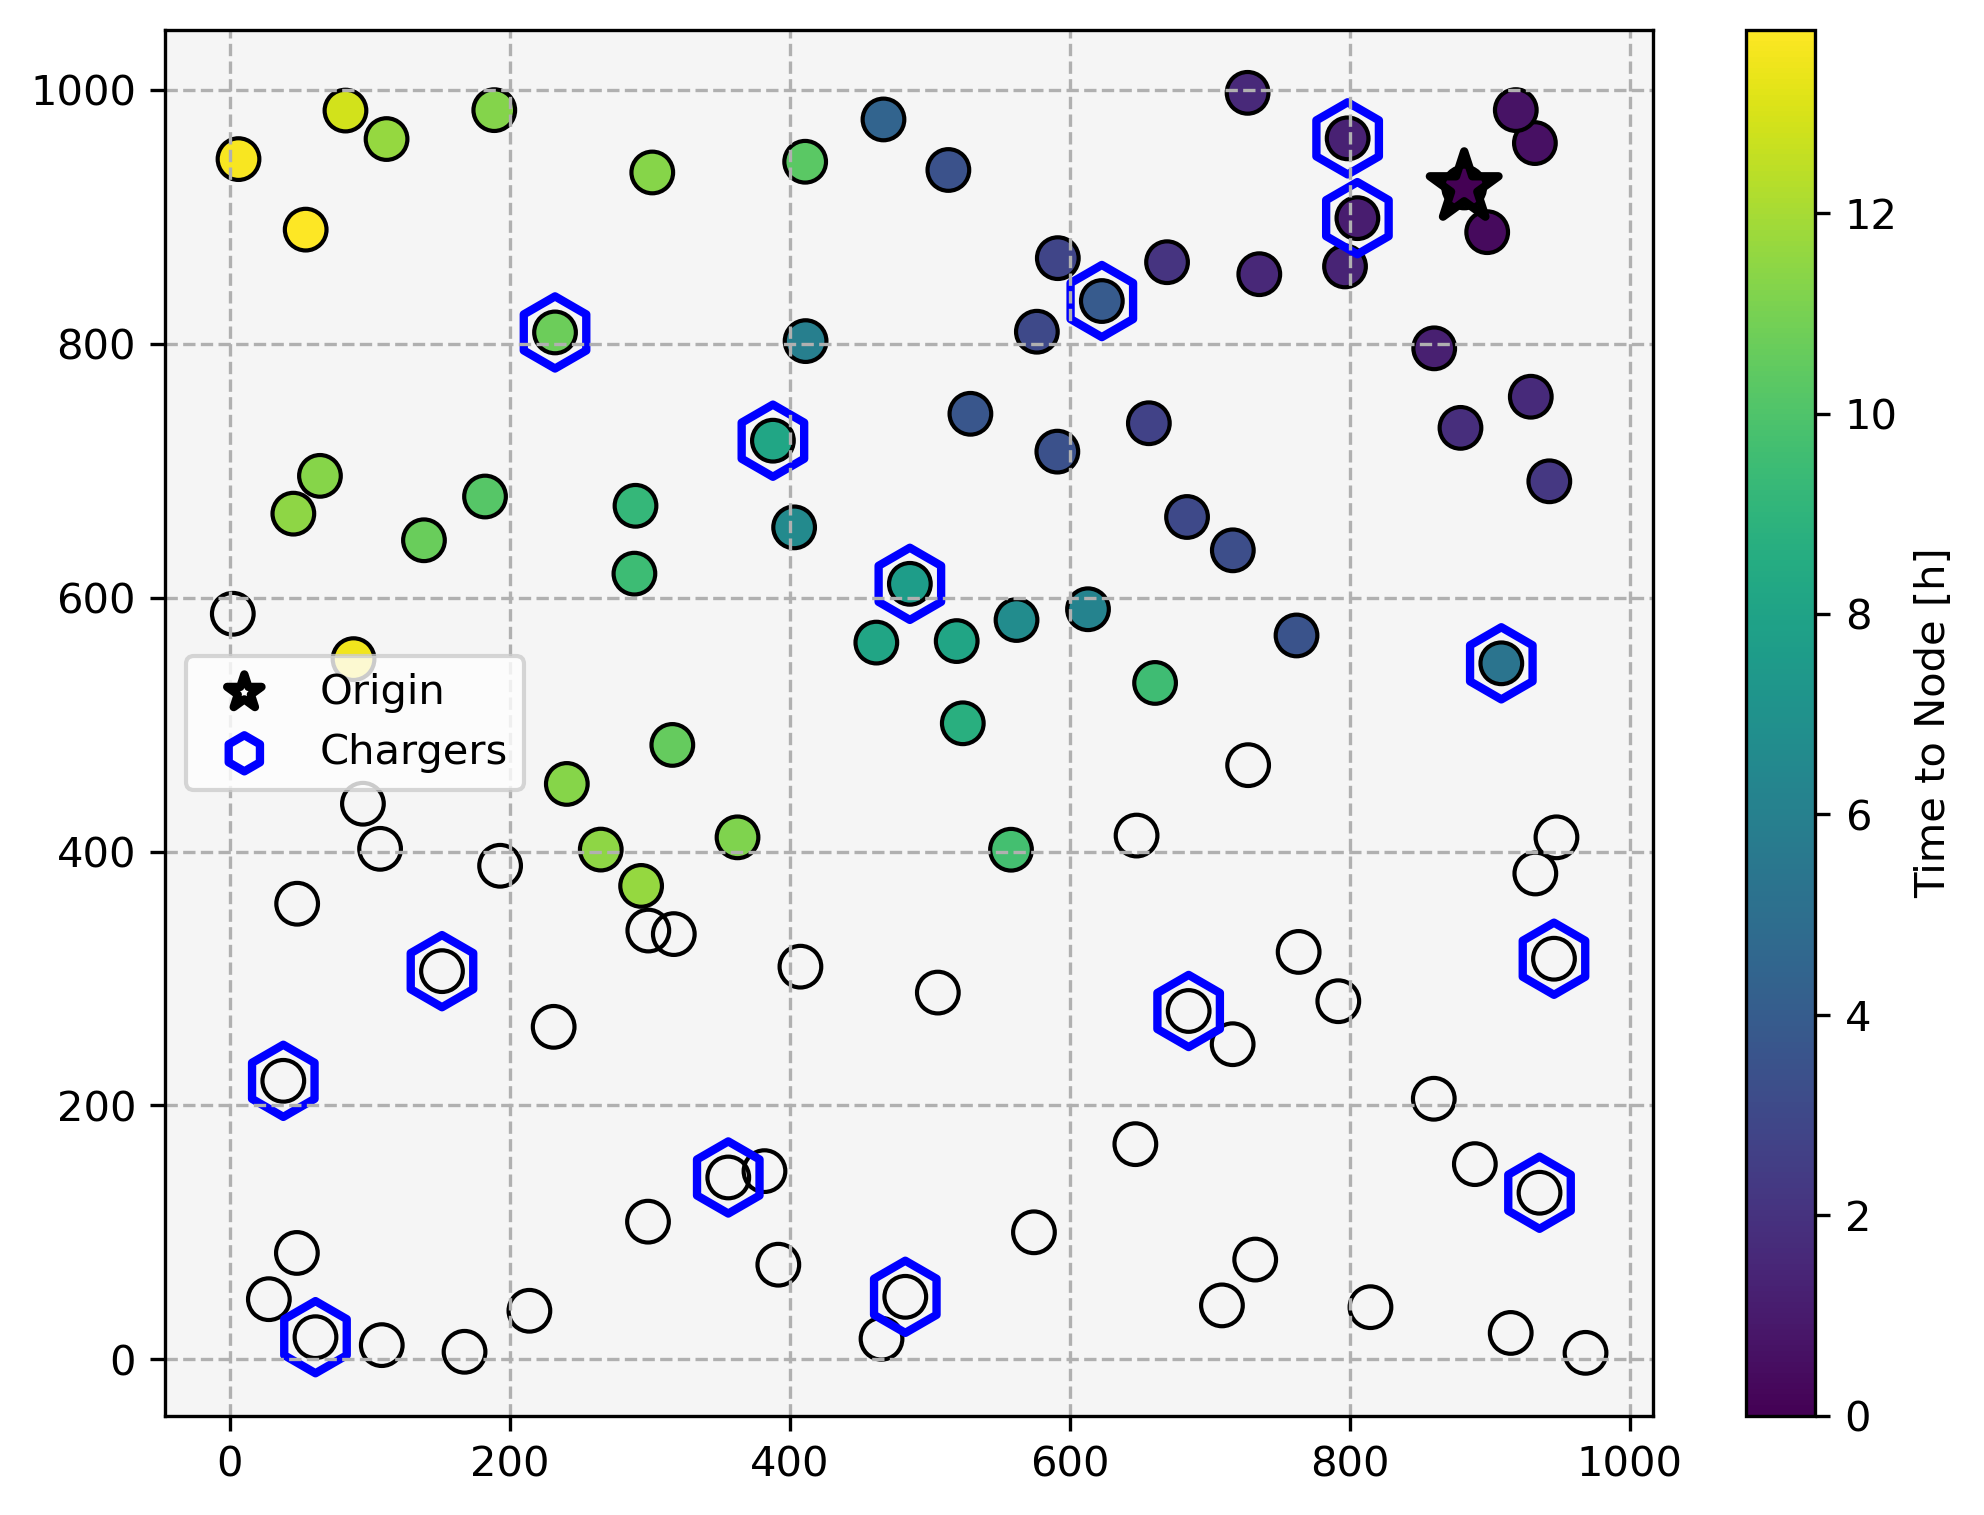
\includegraphics[width = \linewidth]{figs/parameter_factorial_11.png}
		\captionsetup{width=.8\linewidth}
		\caption{Low risk tolerance and low charger reliability ($p = .9,\ \eta = .5)$}
	\end{subfigure}
	\caption{Expected travel times for optimal routes generated by \gls{scramd} for varying charger reliability and driver risk tolerance}
	\label{fig:parameter_factorial}
\end{figure}

As seen in Figure \ref{fig:parameter_factorial} \gls{scramd} optimal routes are effected by both reliability and risk tolerance in an additive manner. The high risk tolerance scenarios in the top row show a small effect of charger reliability which leads to slightly longer travel times. The high reliability scenarios in the first column shows a small effect of risk tolerance, even smaller than the previously mentioned effect. However, the low risk tolerance scenarios in the second row show a huge effect of charger reliability and the low reliability scenarios in the second column show a huge effect of risk tolerance. This result reinforces the need for \gls{scram} - \textbf{the underlying parameters of \gls{pev} charging networks go hand-in-hand with user risk tolerance to effect \gls{pev} dis-utility}.

\subsection{Cost Differential}

If the user experience for \glspl{pev} is different than that for \glspl{icev} the difference is due to charging vs. fueling. Charging a \gls{pev} at a public charging station is, overall, a worse experience than \gls{icev} refueling or low-rate private \gls{pev} charging. The worse experience is due to the longer time required compared to fueling and charger sparsity and unreliability. Although DC charging is, on a cost-per-unit-range-added basis often cheaper than fueling, the pricing structure associated with DC charging is variable and, often, opaque. Gasoline prices, in the US, are determined by individual stations but are, in general, set on the basis of weeks-ahead futures contracts. The price of a gallon of gasoline will be fairly predictable on a several-day timescale and within a region. In effect, most of the time \gls{icev} drivers will have a reasonable expectation that they will be able to find a working fueling station with predictably priced gasoline before running out of fuel when their refueling warning light comes on. It is, however, common for \gls{icev} drivers who are operating in areas which are sparsely populated and/or unfamiliar to them to maintain a higher fuel state by stopping to fuel more often. Comparing the regularity and reliability of the fueling infrastructure present on interstate highways which traverse the emptiest expanses of the American west to the DC charging infrastructure in the most populated portions of the country is a sobering exercise.

The cost-of-travel for a given O/D pair for a given mode is effected by the network structure as well as underlying mode characteristics. If the driving distance for an O/D is considerably less than half of a given vehicle's range then it might be assumed that traversal will not be effected by charging/fueling. For longer trips, wherein charging/fueling is required itinerary cost (time, distance, price) may be directly added by a chartering/fueling event or may be increased due to the need to take a sub-optimal route to accommodate the event. Figure \ref{fig:suboptimal_paths} shows this effect by comparing \gls{bev} travel times with and without charging time included with \gls{icev} travel times for the same graph while assuming that all chargers are always usable and available.

\begin{figure}[H]
	\centering
	\begin{subfigure}[t]{.5\linewidth}
		\centering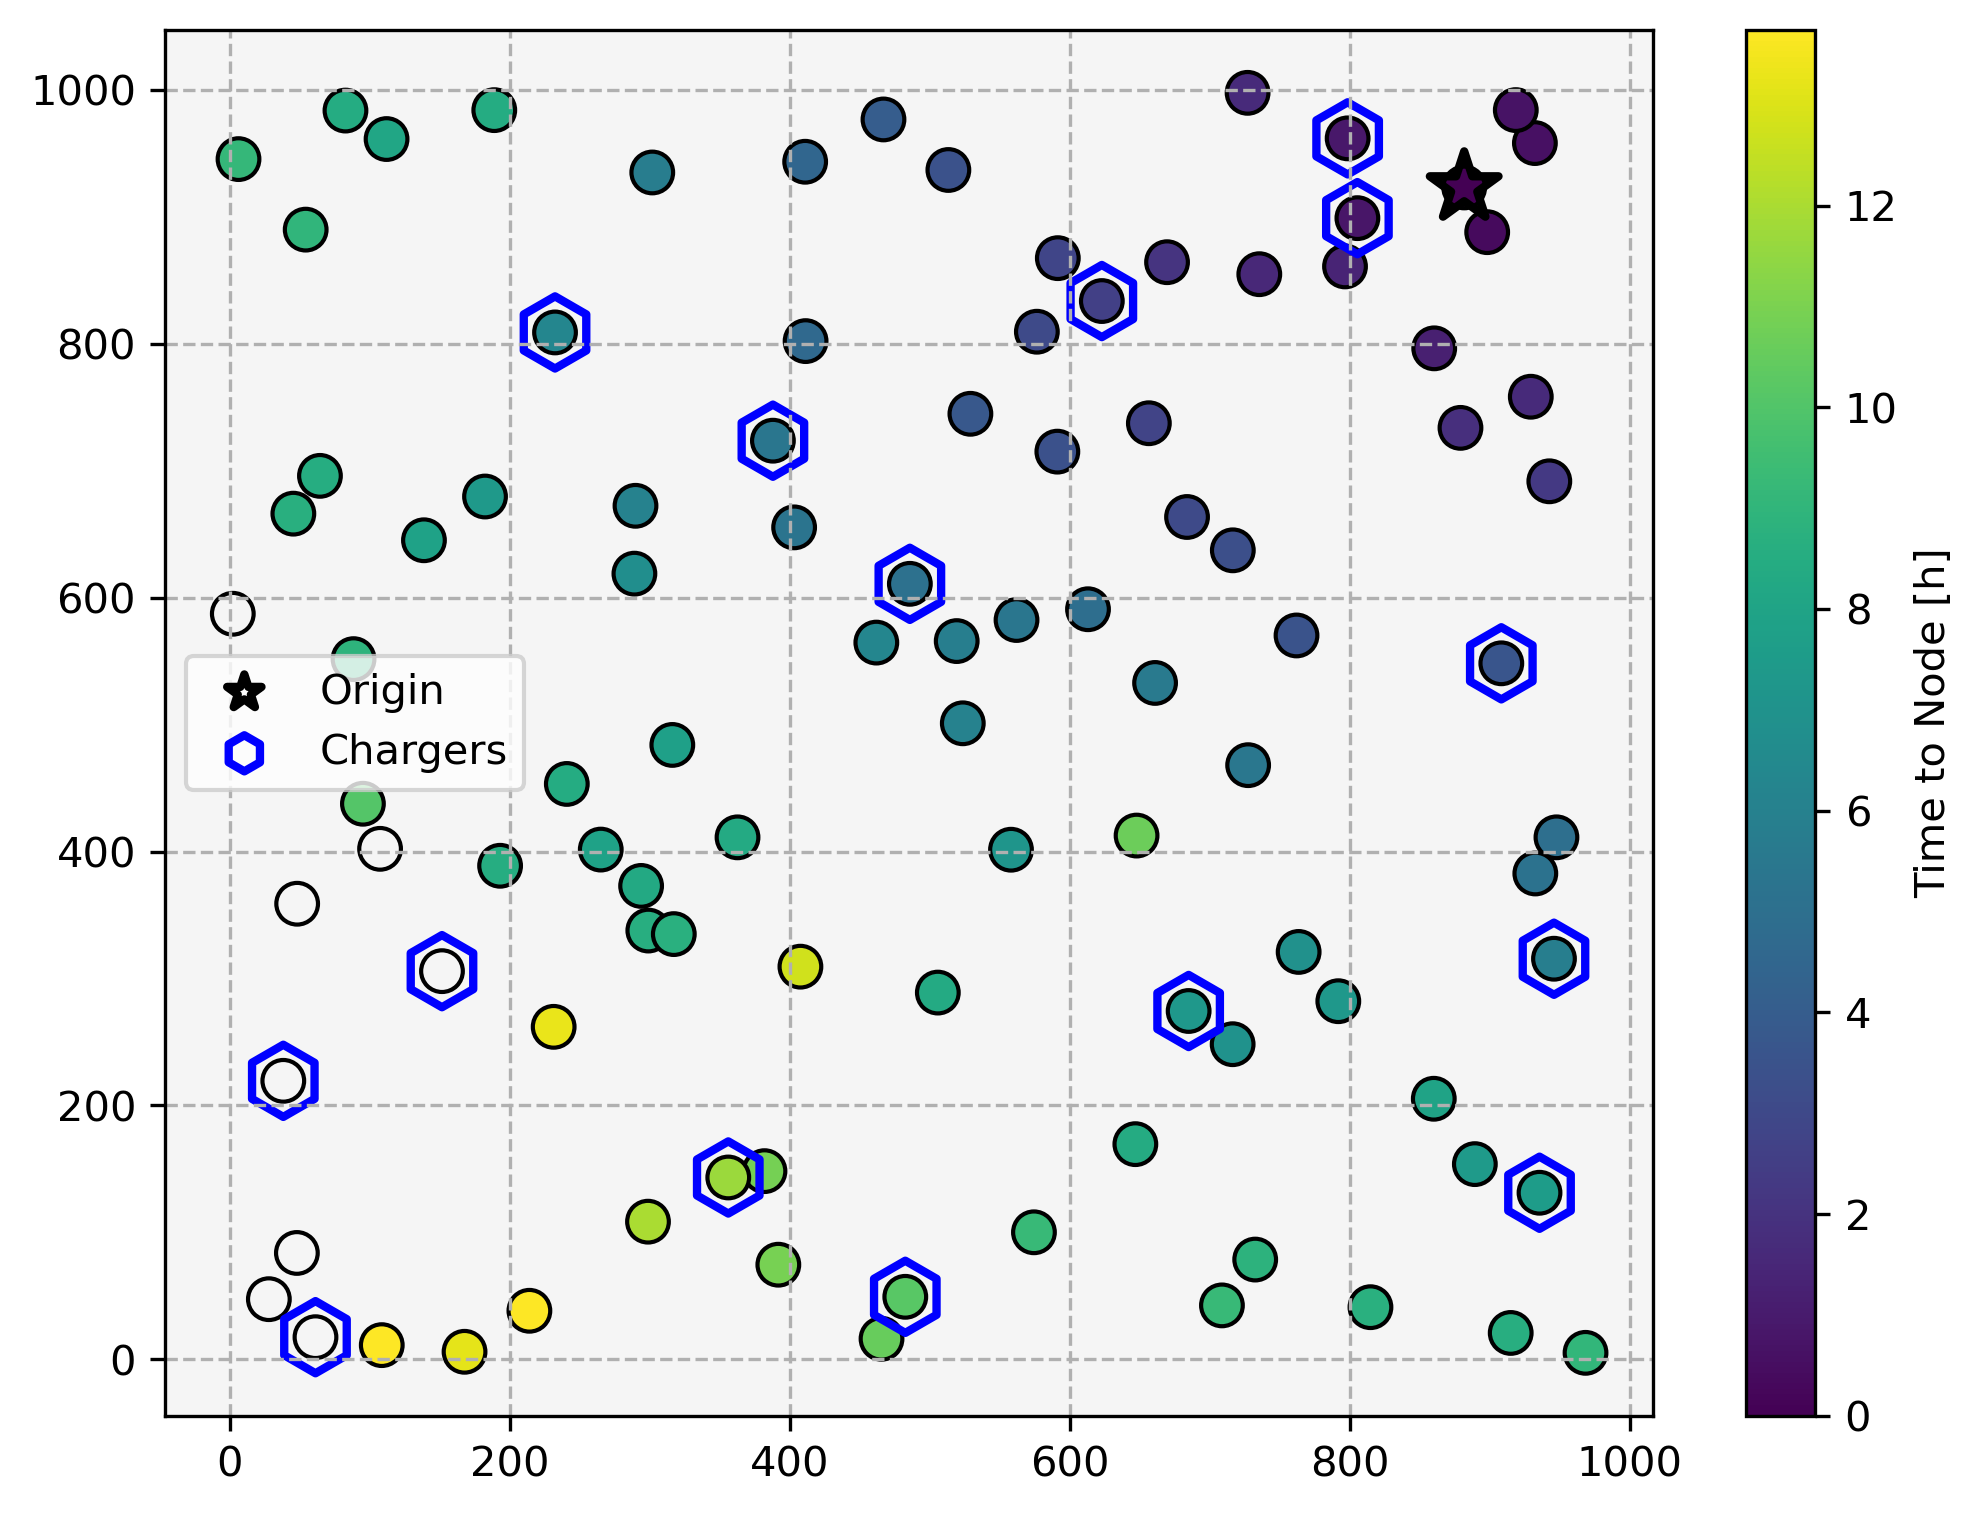
\includegraphics[width = \linewidth]{figs/effect_of_charging_bev_nc.png}
		\captionsetup{width=.8\linewidth}
		\caption{\gls{bev} travel times without charging time}
	\end{subfigure}%
	\begin{subfigure}[t]{.5\linewidth}
		\centering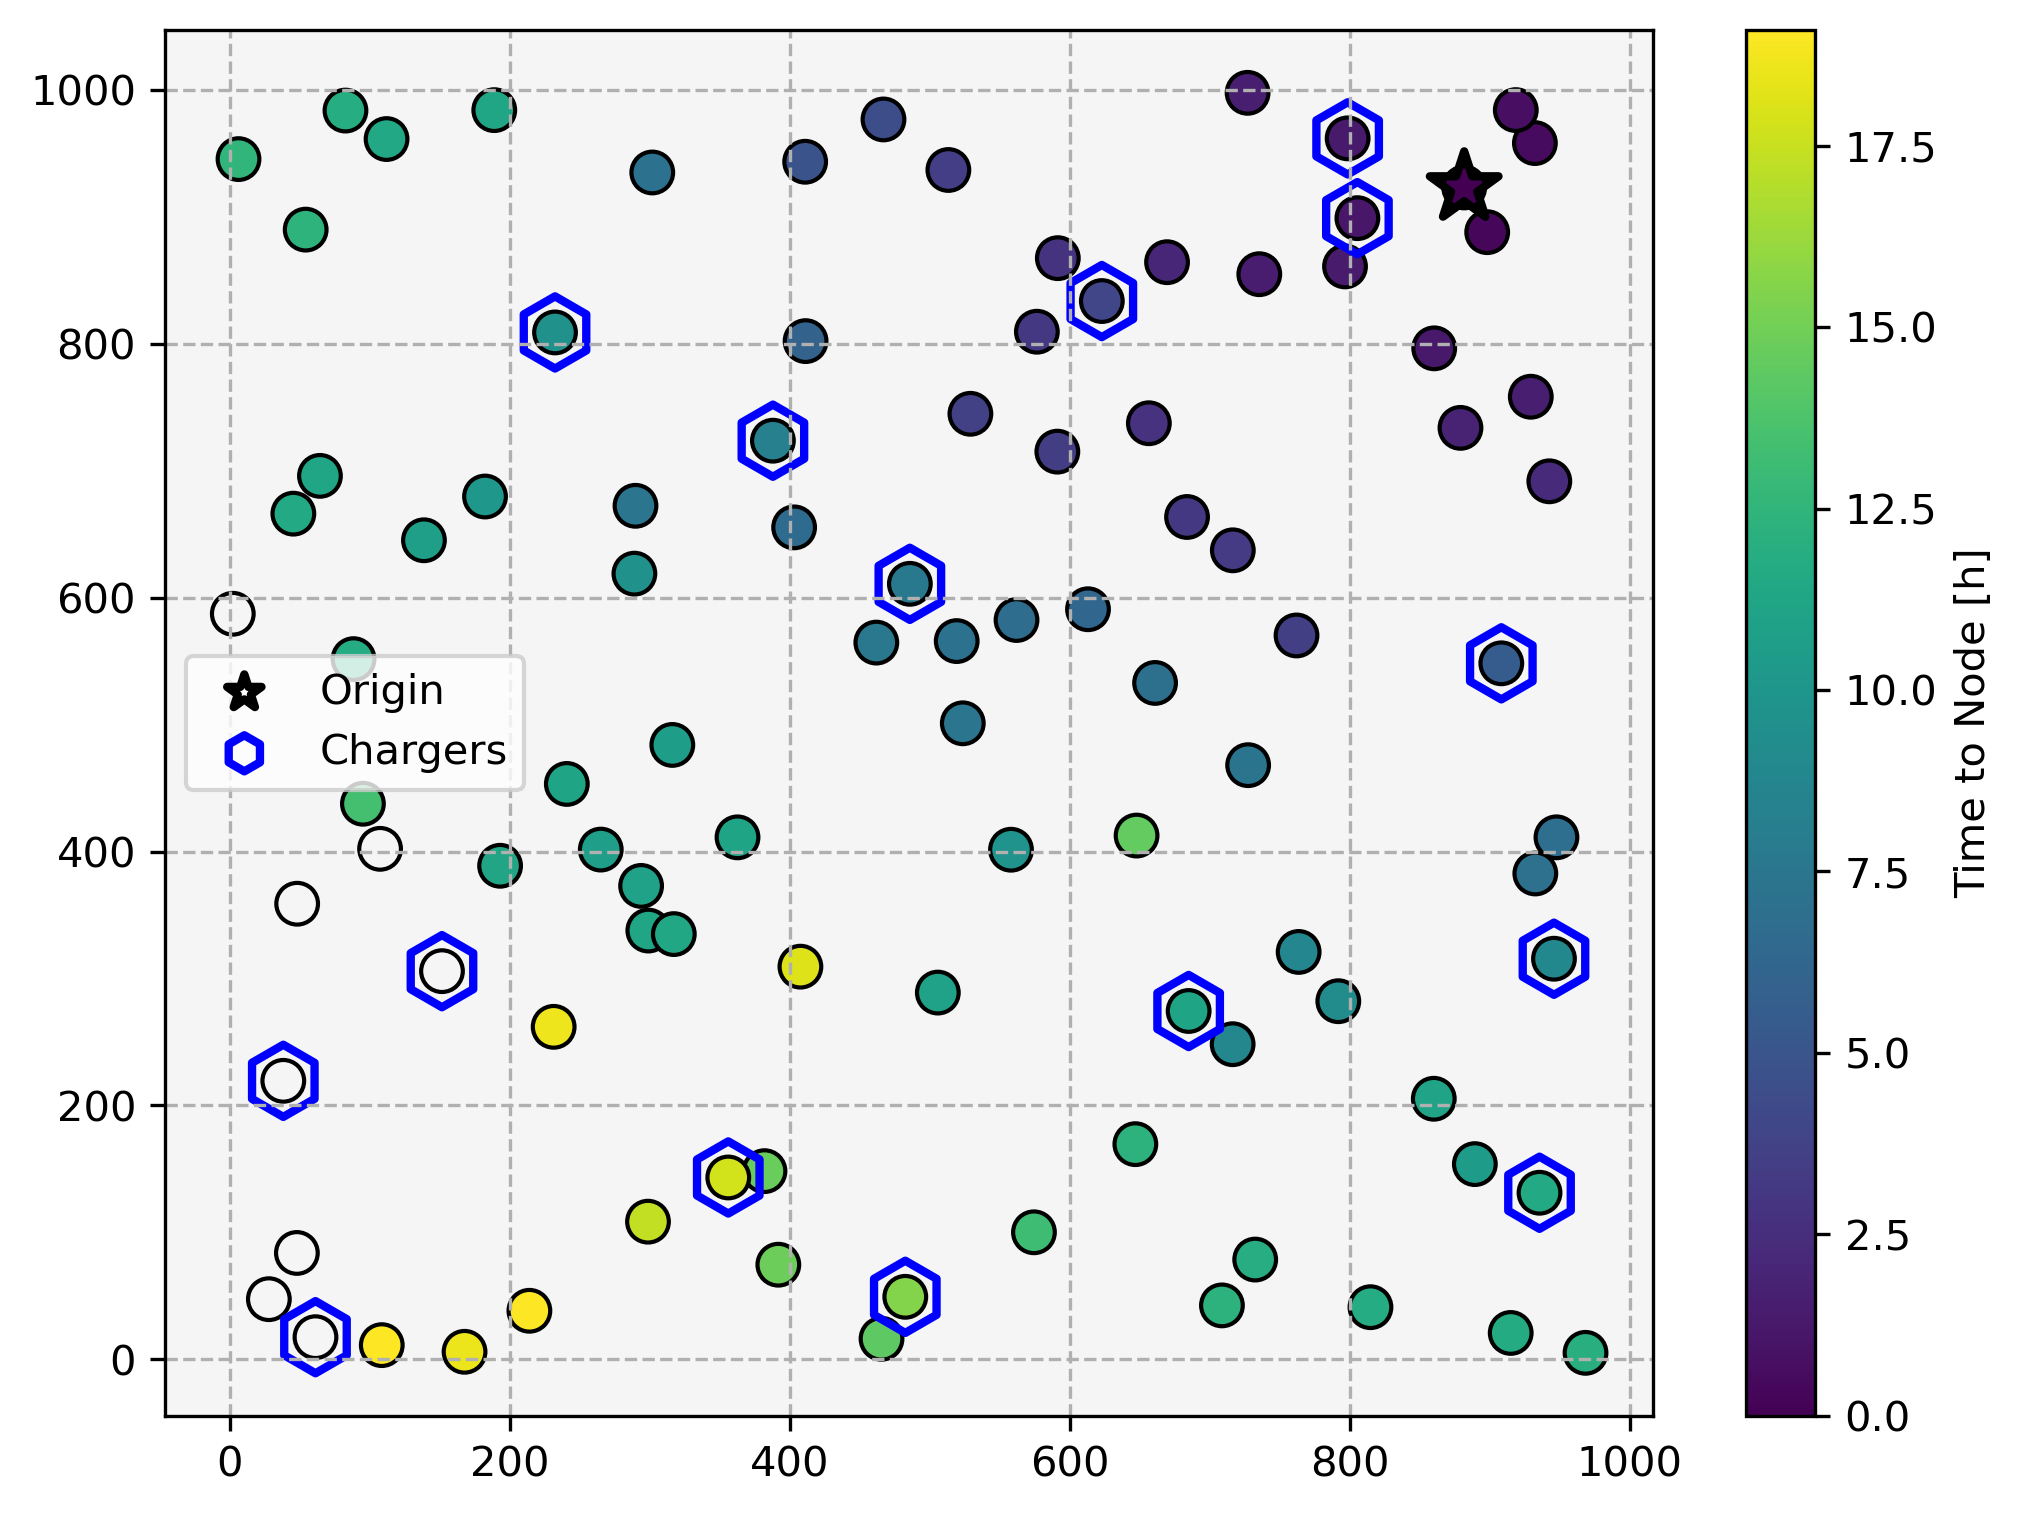
\includegraphics[width = \linewidth]{figs/effect_of_charging_bev_c.png}
		\captionsetup{width=.8\linewidth}
		\caption{\gls{bev} travel times with charging time}
	\end{subfigure}
	\begin{subfigure}[t]{.5\linewidth}
		\centering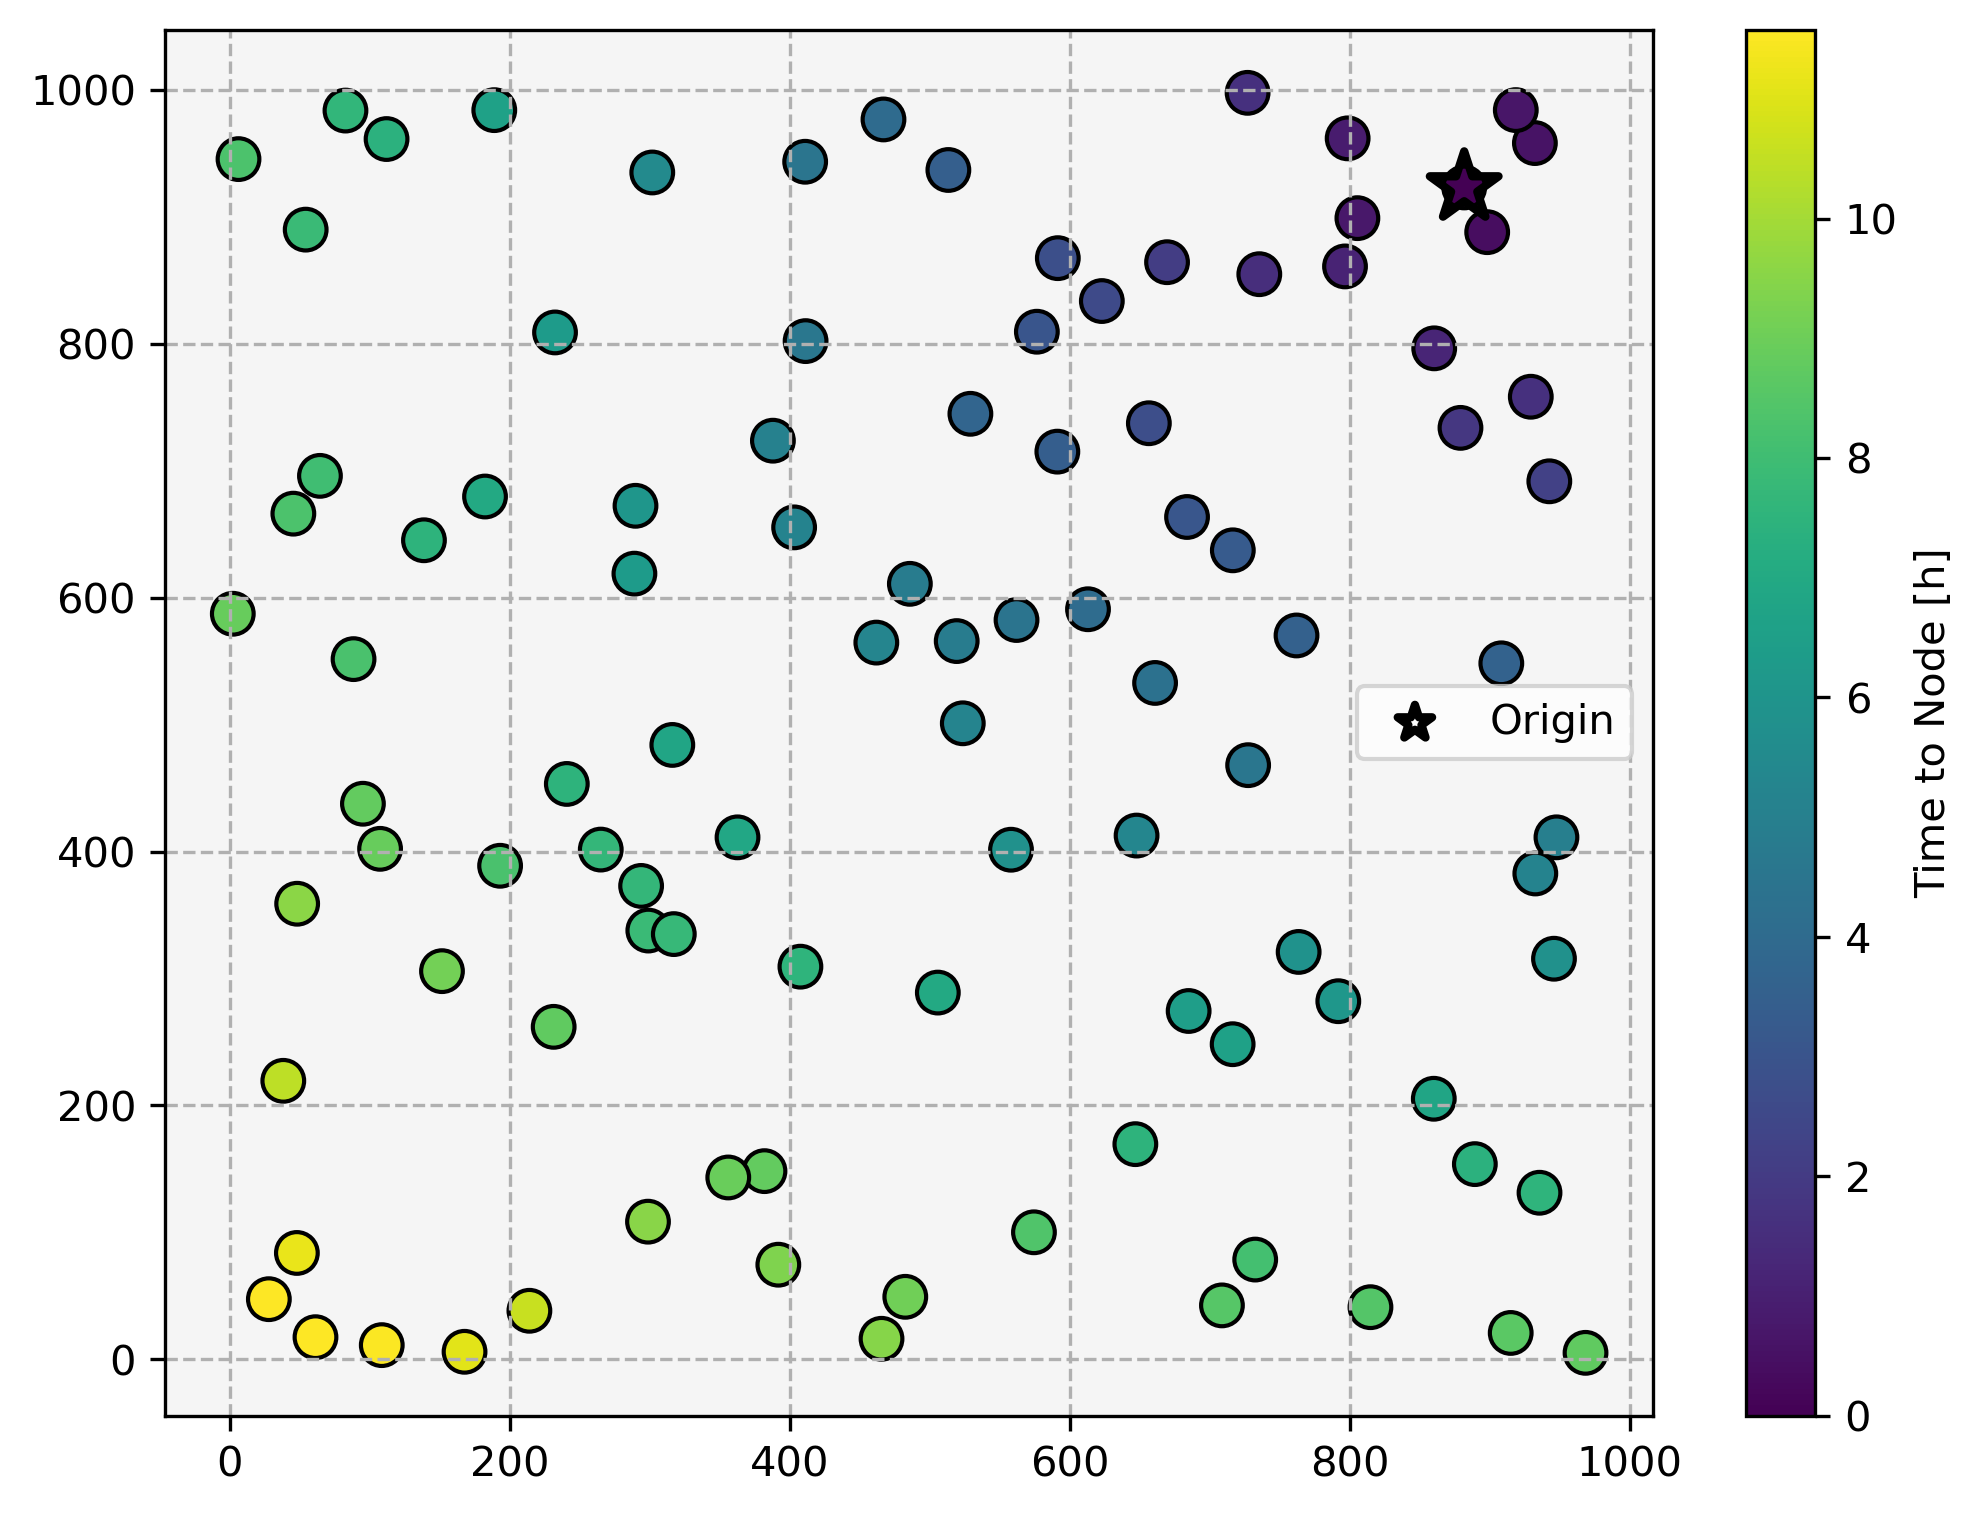
\includegraphics[width = \linewidth]{figs/effect_of_charging_icev_nc.png}
		\captionsetup{width=.8\linewidth}
		\caption{\gls{icev} travel times without fueling time}
	\end{subfigure}%
	\begin{subfigure}[t]{.5\linewidth}
		\centering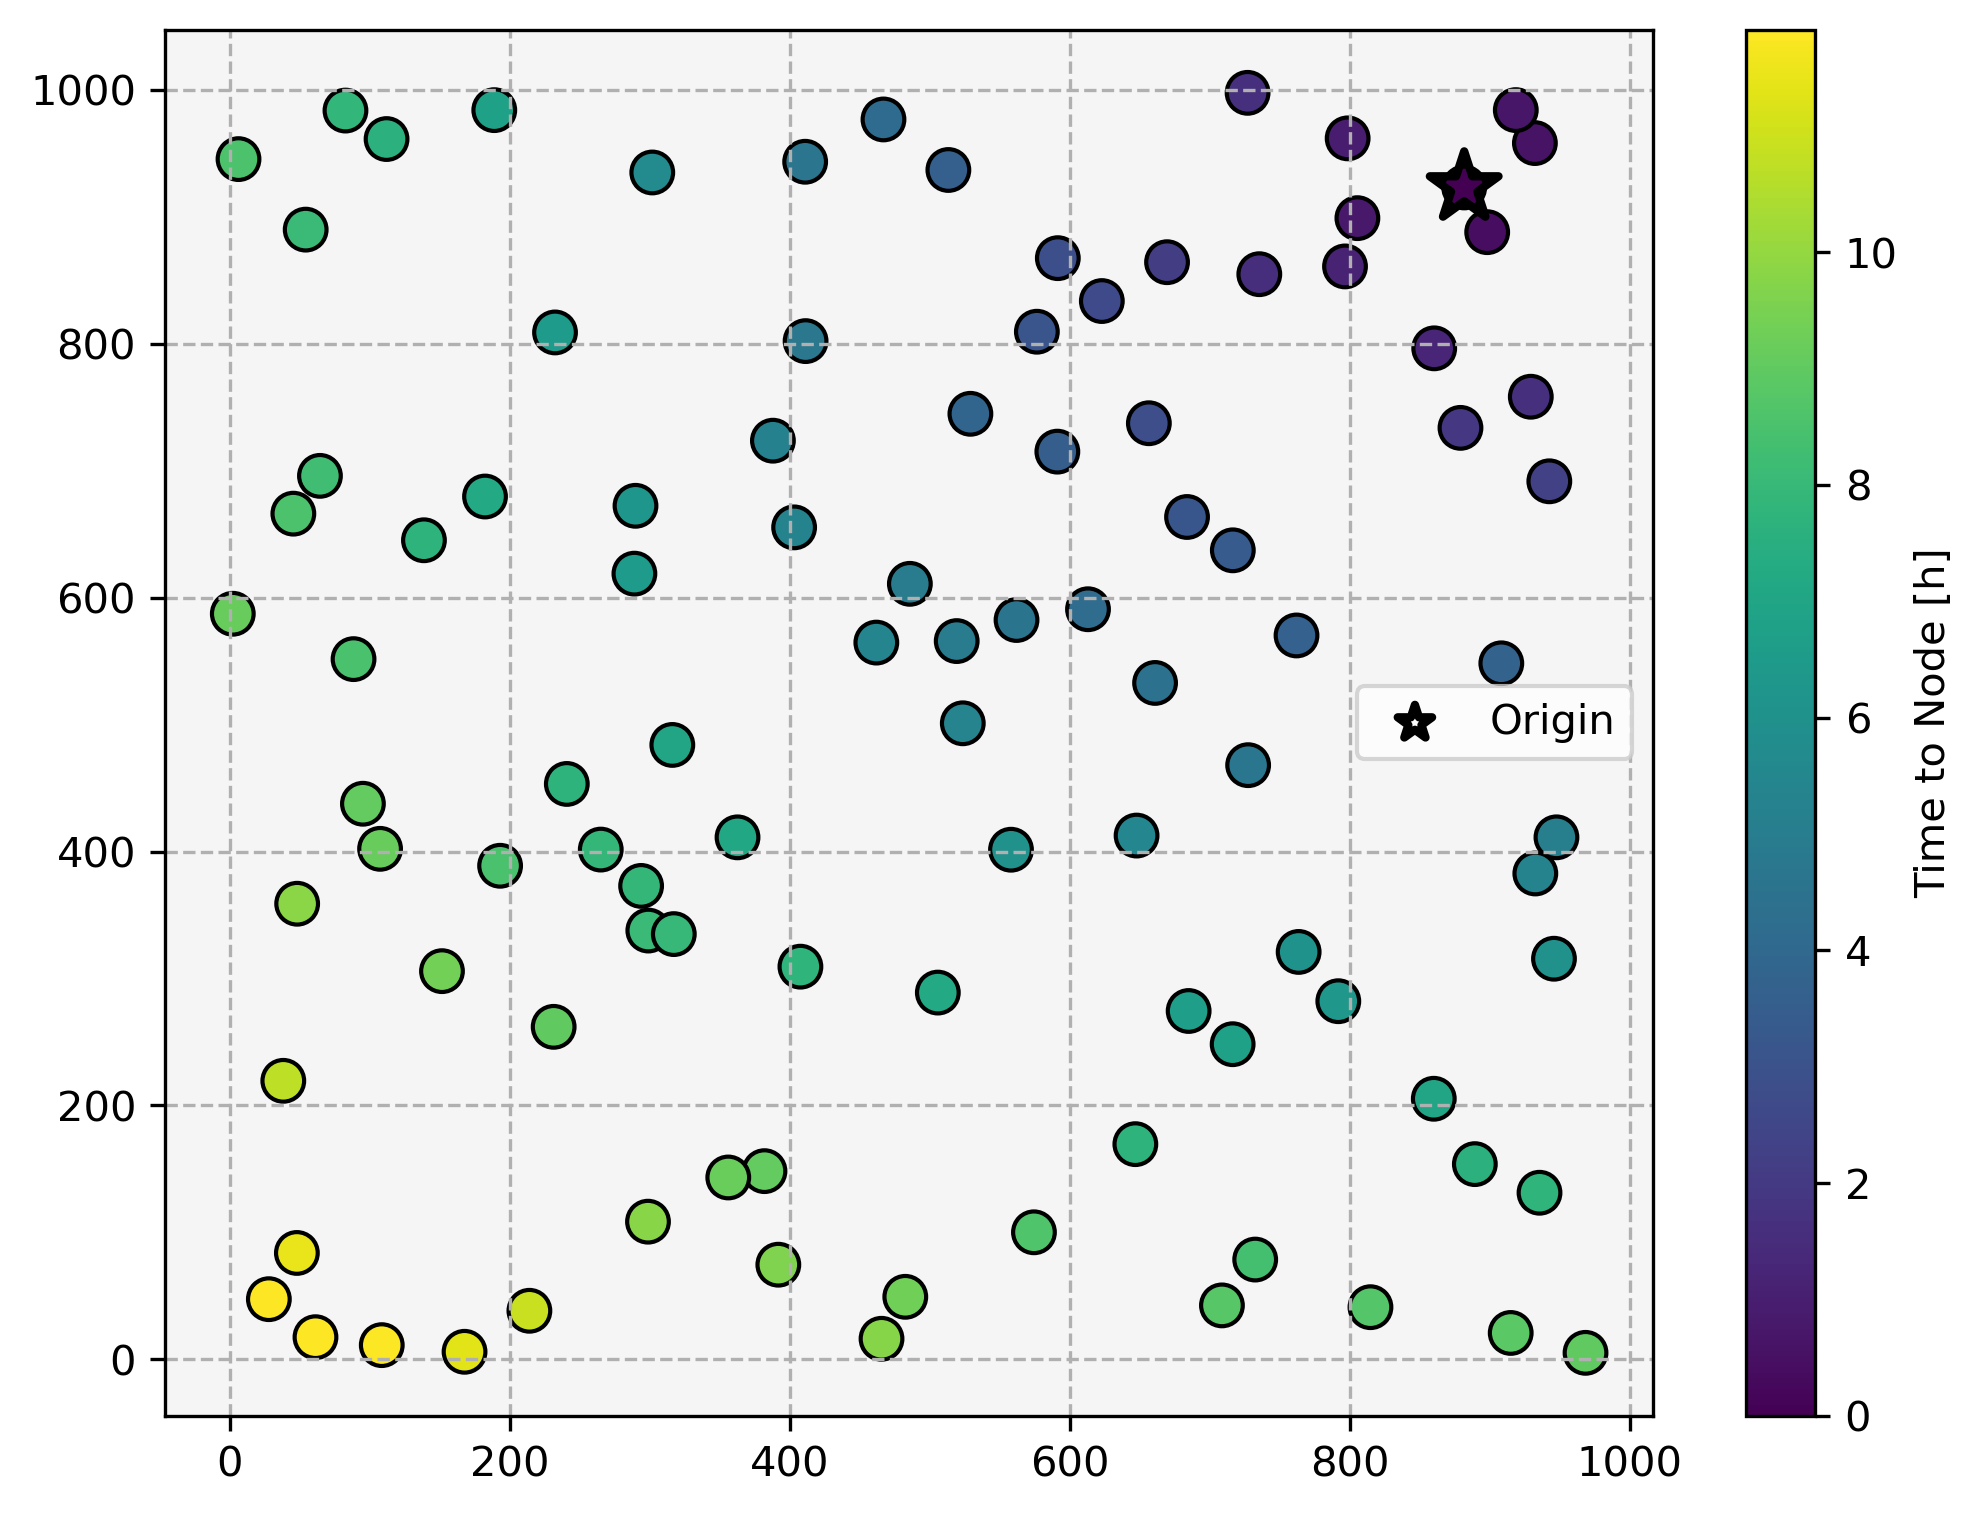
\includegraphics[width = \linewidth]{figs/effect_of_charging_icev_c.png}
		\captionsetup{width=.8\linewidth}
		\caption{\gls{icev} travel times with fueling time}
	\end{subfigure}
	\caption{Expected travel times with and without charging/fueling time included for \gls{bev} with 400 km of range and \gls{icev} with 600 km of range.}
	\label{fig:effect_of_charging}
\end{figure}

In this case the \gls{icev} is assumed to not be effected by limited fueling opportunities and may purchase fuel while pursuing the optimal route. \gls{icev} fueling time and price were modeled on the basis of 30 seconds per gallon (to account for setup time) and \$3.50 per gallon where fueling requirements were assessed. \gls{icev} fueling was assumed to be available at all nodes. The added fueling time for long \gls{icev} trips is not substantial compared to overall trip duration. This is in contrast to the substantial contribution of charging time to overall trip time for long trips taken with \glspl{bev}. However, the limited charger availability compared to fueling stations dictates that equivalent \gls{bev} trips would take longer even if charging was instantaneous. Constrained \gls{bev} routing generally also means longer distance trips following less direct routes which eats into the price advantage provided by \glspl{bev}. Optimal route cost quantiles are shown in Figure \ref{fig:routes_boxplots}.

\begin{figure}[H]
	\centering
	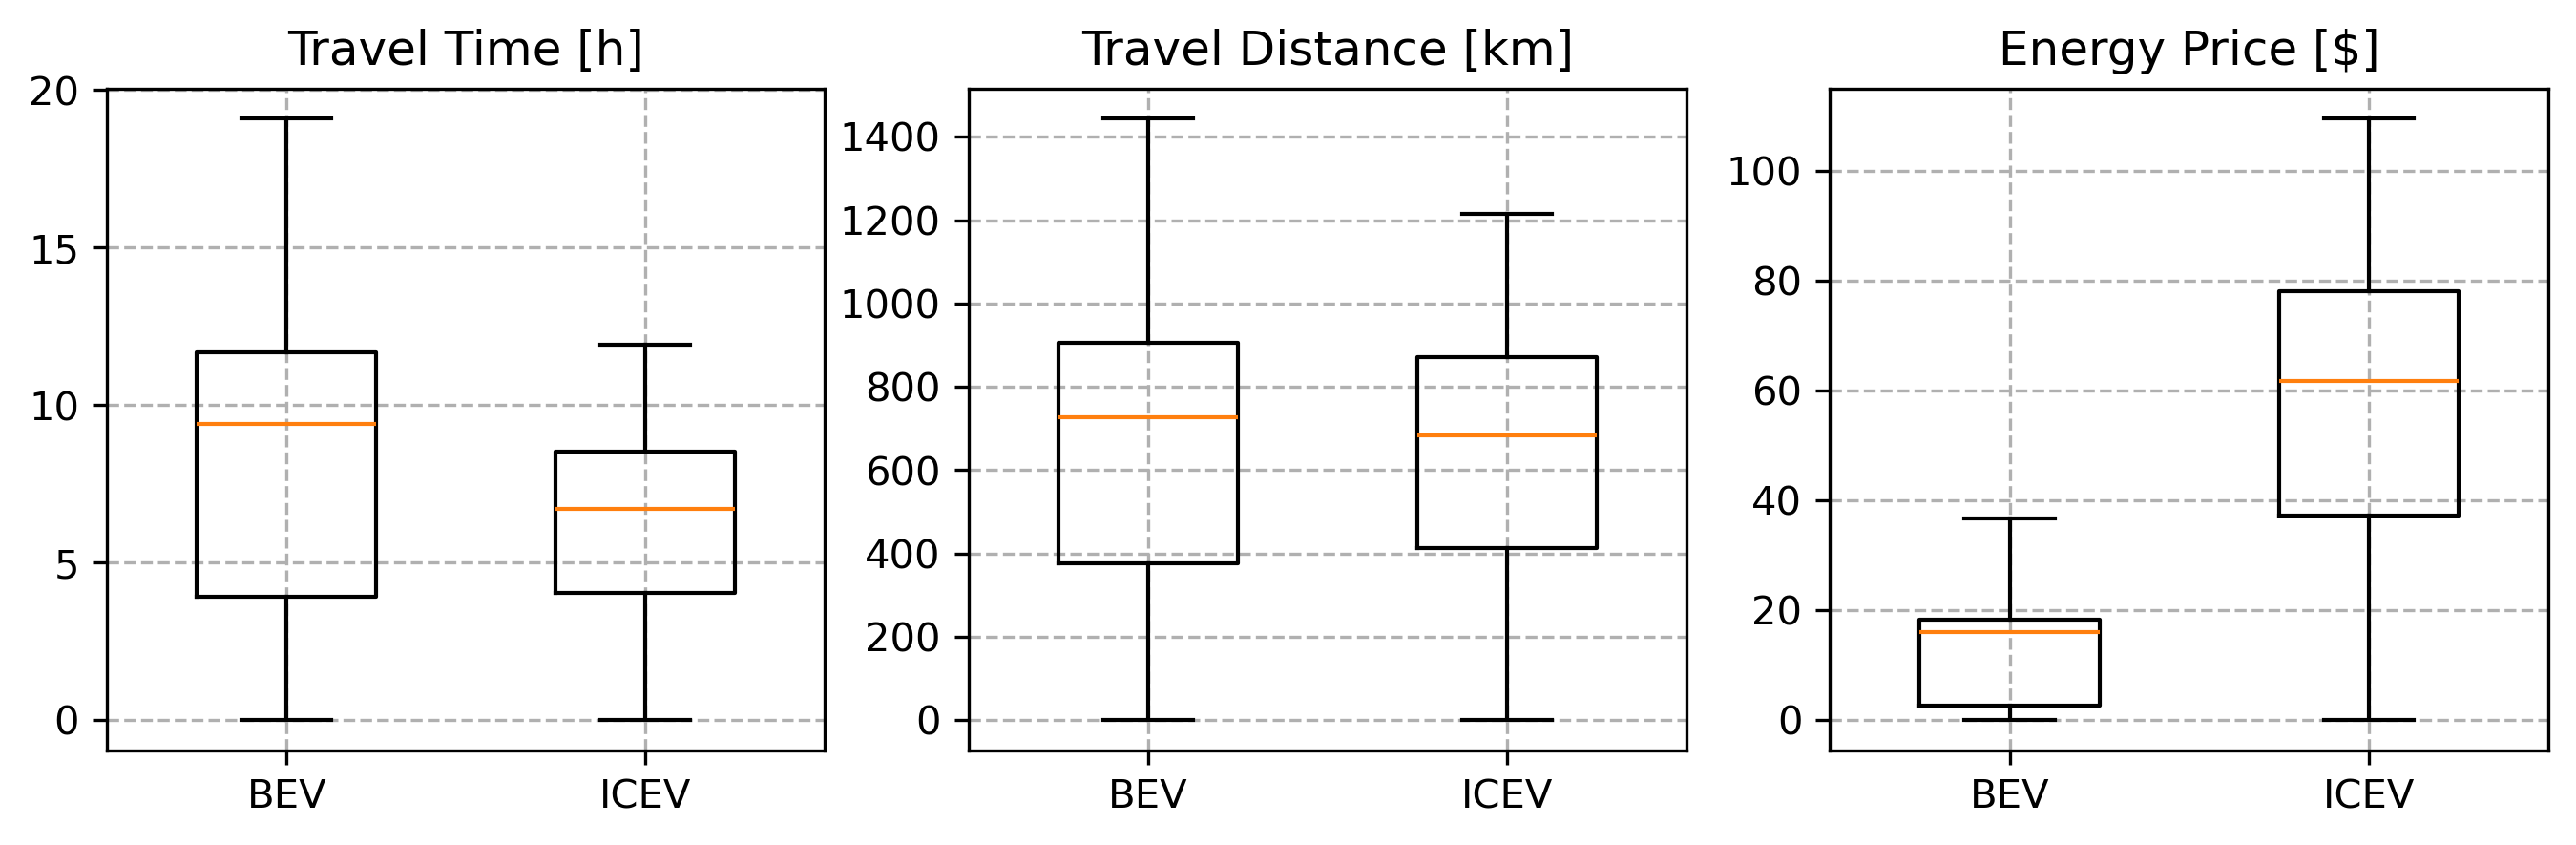
\includegraphics[width = \linewidth]{figs/routes_boxplots.png}
	\caption{Quantiles of costs for optimal routes for \glspl{bev} and \glspl{icev}}
	\label{fig:routes_boxplots}
\end{figure}

While the differential in range-addition rates between charging and fueling is unlikely to be massively reduced in the near future, the influence of charging station location on optimal routing can be reduced by more and better-placed charging stations.